\documentclass{article}

\usepackage{color}
\usepackage[margin=1in]{geometry}
\usepackage{graphicx}
\usepackage{hyperref}
\usepackage{listings}

\definecolor{gray}{rgb}{0.5, 0.5, 0.5}
\definecolor{darkgreen}{rgb}{0, 0.6, 0}

\begin{document}
\raggedright
Homework 1 \break
Christopher Seagraves
% % % % % % % % % % % % % % % % % % % % % % % % % % % % % % % % % % % % % % % % 

    \section*{Problem 1}
        \raggedright
        Orange is the visibility graph... \break
        Green is the reduced visibility graph... \break
        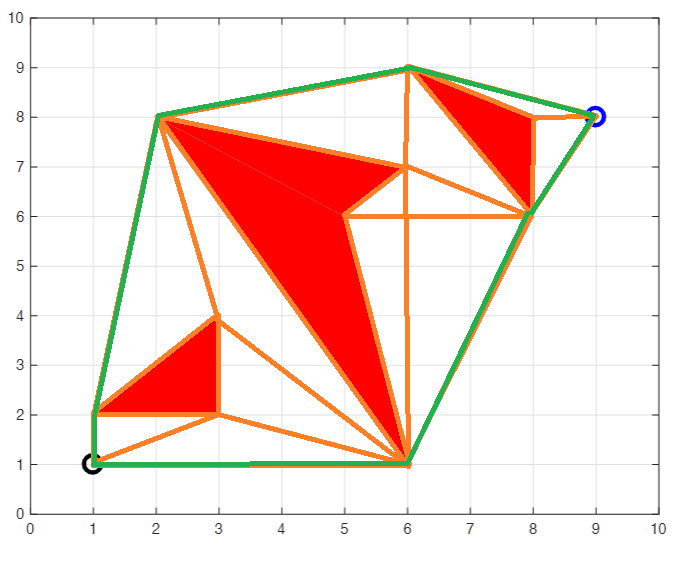
\includegraphics[height=3in]{HW1P1 Visibility Graphs.png}

% % % % % % % % % % % % % % % % % % % % % % % % % % % % % % % % % % % % % % % % 

    \section*{Problem 2}
        \raggedright
        ./Node.py \break
        \url{https://github.com/nosv1/seagraves_unmanned_systems/blob/main/HW1/Node.py}

% % % % % % % % % % % % % % % % % % % % % % % % % % % % % % % % % % % % % % % % 

    \section*{Problem 3}
        \raggedright
        Blue is the shorter path...
        \break
        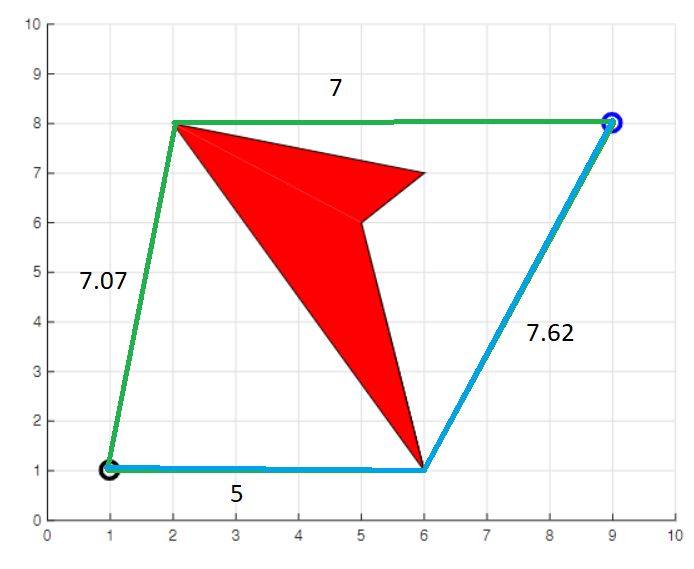
\includegraphics[height=3in]{HW1P3 Reduced Visibility Graph.png}

% % % % % % % % % % % % % % % % % % % % % % % % % % % % % % % % % % % % % % % % 

    \section*{Problem 4}
        \begin{minipage}{\linewidth}
            \raggedright
            ./Grid.py \break
            \url{https://github.com/nosv1/seagraves_unmanned_systems/blob/main/HW1/Grid.py} \break \break
            ./main.py
            \lstset{
                frame=tb,
                language=Python,
                tabsize=4,
                numbers=left,
                basicstyle=\small\ttfamily,
                numberstyle=\tiny\color{gray},
                keywordstyle=\color{blue},
                commentstyle=\color{gray},
                stringstyle=\color{darkgreen}
            }
            \begin{lstlisting}
from Grid import Grid

def main():
    grid: Grid = Grid(
        max_x=10,
        max_y=10,
        grid_spacing=0.5
    )
    grid.plot()

if __name__ == "__main__":
    main()
            \end{lstlisting}
        \end{minipage}
        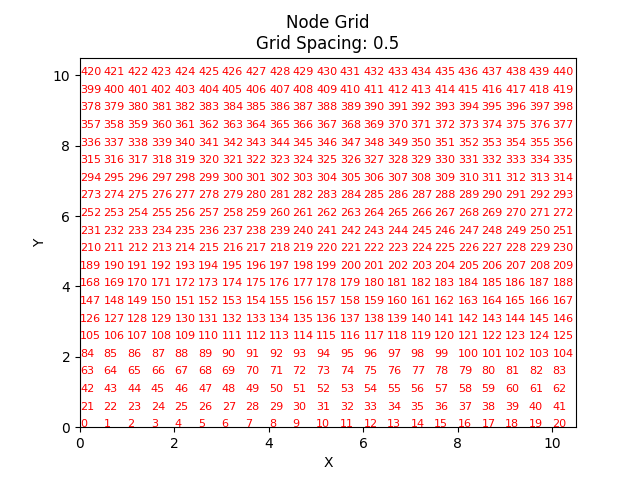
\includegraphics[height=3in]{node_grid.png}

% % % % % % % % % % % % % % % % % % % % % % % % % % % % % % % % % % % % % % % % 

    \section*{Problem 5}
        \begin{minipage}{\linewidth}
            \raggedright
            ./main.py
            \lstset{
                frame=tb,
                language=Python,
                tabsize=4,
                numbers=left,
                basicstyle=\small\ttfamily,
                numberstyle=\tiny\color{gray},
                keywordstyle=\color{blue},
                commentstyle=\color{gray},
                stringstyle=\color{darkgreen}
            }
            \begin{lstlisting}
from Node import Node

def main():
    nodes = [
        Node(2, 1),
        Node(3, 2),
    ]
    distance = nodes[0].distance(nodes[1])  
    print(f"Distance: {nodes[0].distance(nodes[1])}")
    
if __name__ == "__main__":
    main()
            \end{lstlisting}
            Outputs: \break
            Distance: 1.4142135623730951
        \end{minipage}

% % % % % % % % % % % % % % % % % % % % % % % % % % % % % % % % % % % % % % % %

\end{document}